%%
%% Author: jamie
%% 05/10/18
%%
\chapter{Implementation}\label{ch:development}
In this chapter the details of the product developed will be discussed.
This includes the implementation of the MCTS algorithm, our metric computation and
the development of our prototype game for demonstration purposes.


\section{Smooth UCT Algorithm}\label{sec:MCTS}
The core component of our implementation is the smooth UCT algorithm, as
outlined in section 2.4.
As such, in this section, the code corresponding to this algorithm will be outlined.

\subsection{Tree Representation and Utility Functions}\label{subsec:treeRepresentation}
This subsection seeks to provide background on the data structures implemented and some
of the functions heavily utilised in the following chapter.
These are not core elements of the algorithm and thus \textbf{the reader may choose to skip
to section 3.1.2}.

\subsubsection{Histories}
As mentioned in section 2.1.2, when dealing with a POMDP, we must use histories to represent states.
These histories consist of a sequence of actions and observations\citep{silver2010monte}.
When practically applied to the game of Leduc Hold'em this means that we must store all of the
cards dealt and the actions taken as a part of each history.
In order to store history information in a simple, parsable manner it was decided that strings would be used.
Their primary components would be cards and actions.
In order to simplify the data involved abbreviations were used for both cards and actions.
Below is the list of abbreviations for cards:

\begin{itemize}
    \item \textbf{Ah} - Ace of Hearts
    \item \textbf{As} - Ace of Spades
    \item \textbf{Kh} - King of Hearts
    \item \textbf{Ks} - King of Spades
    \item \textbf{Qh} - Queen of Hearts
    \item \textbf{Qs} - Ace of Spades
\end{itemize}

Below is the list of abbreviations for actions:
\begin{itemize}
    \item \textbf{f} - Fold
    \item \textbf{c} - Call
    \item \textbf{b} - Bet
    \item \textbf{r} - Raise
\end{itemize}

The final component required to represent a history was a prefix.
The prefix corresponds to the player that is first to play in the game and facilitates the computation of
the next player to take an action given any history.
In our case, it could be either 1 or -1.
The table below gives a full breakdown of an example history.

\addvbuffer[12pt 12pt]{\begin{tabular}[ht]{ | p{2.5cm} | p{2.5cm} | p{2.5cm} | p{2.5cm} | p{2.5cm} |}
      \hline \textbf{Prefix} & \textbf{Private Cards} & \textbf{Round 1 Actions} & \textbf{Public Cards} & \textbf{Round 2 Actions}\\
      \hline
       1 & AhQh & bc & Ks & brc\\
      \hline
\end{tabular}}

\subsubsection{Game Tree}
The tree data structure consists of two primary components: histories and nodes.
A python dictionary was used with the keys being histories and the values being nodes.
Nodes were defined as simple data structures that contained a visitation count, a value,
a parent and a set of children.
Both the parent and the children were histories that also existed as keys in the
tree dictionary thus facilitating $\mathcal{O}$(1) lookup time.

\begin{lstlisting}[style=Python]
class PoNode:

    def __init__(self):
        self.visitation_count = 1
        self.value = 0
        self.parent = ""
        self.children = set()

# Example instantiation.
# In our implementation the root node was was an empty string.
tree = {"": PoNode()}
\end{lstlisting}

\subsubsection{Strategies}
In the rest of the chapter different types of strategies are discussed.
Specifically, we refer to deterministic and stochastic strategies.

When referring to deterministic strategies we mean strategies that have a single
action associated with each state or history.
This means that whenever that history is reached the same action will be selected each time.
In the implementation, these strategies are derived by analysing the values of nodes in the game tree.
The action that is taken at any given history is the action that will lead us to the child whose
value is the highest.

Stochastic strategies are strategies that provide a probability distribution across the available actions
at a given state or history.
This means that each action may be taken at a particular history but, there is a different probability
of taking each action.
These strategies are derived as a direct result of the average strategy used by the agent.
In other words, the visitation counts of nodes during the MCTS training.
Due to the fact that MCTS samples states at a biased rate based on the expected value of the state we
can use this information to induce stochastic strategies.
This process is outlined in more detail in section 2.4.3.

\subsubsection{Utility Functions}\label{subsec:utility}
The first utility function is the util.terminal function.
This function corresponds to the TERMINAL function listed in Algorithm 1 and
takes a history as an argument returning a boolean value.
For example, if a player has folded then the return will be true.

The second utility function is the util.player function.
This corresponds to the PLAYER function listed in Algorithm 1, again taking a history as it's sole argument.
Depending on who is next to act it will return 1(player 1), 0(dealer) or -1(player 2).

The final utility function that will be discussed is the util.information\_function.
This function corresponds to the information function, $I$, in Algorithm 1.
It is parameterised by a player and a full game history.
The return value is that same history without the opponent's private card
embedded in the history.
For example passing parameters ("1AhQhbc",1) would return "1Ahbc".
Note that the second card "Qh" has been stripped from the returned history.

\subsection{Selection}\label{subsec:selection}
The python implementation for Smooth UCT action selection was a relatively close approximation of the
algorithmic SELECT function as discussed in section 2.4.
The first distinction that should be made is that in section 2.4 states and information
states were mentioned when discussing the Smooth UCT algorithm.
In this chapter histories and player histories will be discussed as parallel concepts in the implementation.
Another notable difference is that instead of storing the history values and visitation
counts in separate $Q$ and $N$ functions these functions are embedded within the tree data
structure.
This means that when the functions at line 11 and 13 are called these
functions directly correspond to lines 7 and 9 in Algorithm 3.
Due to the fact that these functions are relatively large despite serving a trivial
purpose they have been omitted for brevity.

\begin{lstlisting}[style=Python]
def select(history):
    player = util.player(history)
    player_history = util.information_function(history, player)
    tree = get_tree(player)

    eta_sub_expression = math.pow(1 + d * math.sqrt(tree[player_history].visitation_count), -1)
    eta = max((GAMMA, ETA_ZERO * eta_sub_expression))

    z = random.uniform(0, 1)
    if z < eta:
        return get_best_action_ucb(player_history, tree)
    else:
        return get_action_avg_strategy(player_history, tree)
\end{lstlisting}


\subsection{Expansion}\label{subsec:expansion}
Due to the fact that\citep{heinrich2017reinforcement} did not discuss the details of his EXPANDTREE
function (see Algorithm 1), it was decided that the expansion method detailed
in\citep{silver2010monte} would be used.
This was the original paper that outlined the method of applying MCTS to POMDPs so it seemed
an adequate alternative.
Silver's method stated that all available child nodes would be appended as children to the node to be expanded.
The resulting code is listed below.

\begin{lstlisting}[style=Python]
def expand(tree, history):
    player = util.player(history))
    player_history = util.information_function(history, player)

    if player_history not in tree:
        tree[player_history] = potree.PoNode()

    for action in util.get_available_actions(player_history, player=player):
        new_history = player_history + action
        if new_history not in tree:
            tree[new_history] = potree.PoNode()
        tree[player_history].children.add(new_history)
\end{lstlisting}


\subsection{Simulation}\label{subsec:simulation}
In this section, we will discuss the python equivalents to the ROLLOUT and SIMULATE functions from Algorithm 1.

In the python implementation, the rollout policy, $\pi_{rollout}$, is simply a random policy(line 2).
This means that each action that is available in that state/history has the same probability of being selected.
Furthermore, the state transition function, $G$, is replaced by line 3 below.
This is because the child of a history will always be an action appended to that history.

\begin{lstlisting}[style=Python]
    def rollout(history):
    action = random.choice(util.get_available_actions(history))
    new_history = history + action
    return simulate(new_history)
\end{lstlisting}

The SIMULATE function, when ported to python code had a number of modifications.
First, a tree function is introduced.
This function has the purpose of returning the tree relevant to the current player.

It was also found that an additional condition had to be added for the if statement at line 11.
This condition ensured that the player history had children.
If it did not then the else block would be executed and those children would be added.
During the initial implementation of the algorithm, it was found that the tree would become
disconnected if this condition was not present, with every second layer of the tree having no children.

The final divergence from Algorithm 1's SIMULATE function is the conditional on line 14.
In the case of our implementation, the player can be either of the active players or the dealer.
If the current player is the dealer then we do not want to call the expand function,
nor set the OUT-OF-TREE property to true.

\begin{lstlisting}[style=Python]
def simulate(history):
    if util.is_terminal(history):
        return handle_terminal_state(history)

    player = util.player(history)
    if out_of_tree[player]:
        return rollout(history)

    player_history = util.information_function(history, player)
    player_tree = tree(player)
    if player_history in player_tree and player_tree[player_history].children:
        action = select(history)
    else:
        if player != DEALER:
            expand(player_tree, history, player)
            out_of_tree[player] = True
        action = random.choice(util.get_available_actions(history))

    new_history = history + action
    running_reward = evaluator.calculate_reward_full_info(history) + \
                         discount_factor * simulate(new_history)
    update_player_tree(history, action, player, running_reward)

    return running_reward
\end{lstlisting}


\subsection{Tree Update}\label{subsec:treeUpdate}
The tree update function is essentially identical to the function listed in Algorithm 2 with
the only difference being that the $Q$ and $N$ are embedded in the game tree.
The code is listed below.

\begin{lstlisting}[style=Python]
    def update(tree, history, new_history, running_reward):
    tree[history].visitation_count += 1
    tree[new_history].visitation_count += 1
    tree[new_history].value += (running_reward - tree[new_history].value) / tree[new_history].visitation_count
\end{lstlisting}


\section{Exploitability Computation}\label{sec:bestResponseComputation}
In order to evaluate the performance of our agent exploitability was utilised as the primary metric.
Exploitability is a measure of how well our agent would fare against an opponent responding
optimally to our strategy, ie an opponent using a best response strategy.
Exploitability is related to the concept of Nash equilibria in that a Nash equilibrium
is induced by a strategy that cannot be exploited.
In this section we will discuss the process of calculating exploitability step by step and giving coding examples.
In order to do so we will refer to three player's that are related to the process.
These are the best response(BR) player, the MCTS player and the chance player.
The BR player is the player who's strategy we are attempting to establish through computation
of the best response strategy.
The MCTS player is the player whose strategy has already been established through execution of the MCTS algorithm.
The chance player is the player who is responsible for the chance actions of the game ie dealing cards.

\subsection{Generating Best Response Tree}\label{subsec:applyMCTS}
To calculate the exploitability of a strategy the best responses to that strategy must be
determined.
In other words, the best response strategy must be established.

There are two steps involved in this process.
The first step involves generating a full game tree.
This can be implemented as a relatively trivial recursive function in which we begin at the root of the
tree and at each level add every possible child node until a terminal node is reached.
It is worth noting that the tree generated is a full game tree.
This means that all of the game information is represented in the tree.
As a result, if we wish to view the nodes or histories in the tree from either player's perspective we must apply
the information function in order to remove the opponent's private information from view.
The distinction between the full game tree and the player's information set is illustrated
in figure 3.1.

\begin{figure}[!ht]
    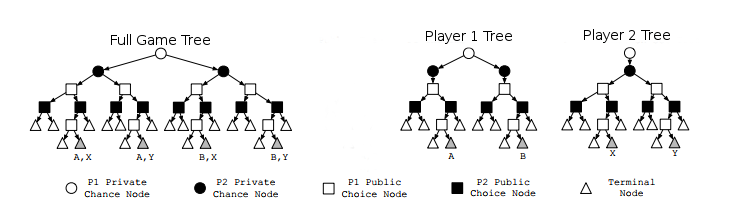
\includegraphics[scale=.6]{images/separate_game_trees_johanson.png}
    \caption{Full Game Tree vs Player Information Set - adapted from\citep{johanson2011accelerating}}
\end{figure}

The code is listed below.

\begin{lstlisting}[style=Python]
def build_tree(history, tree):
    tree[history] = potree.PoNode()

    if not util.terminal(history):
        actions = util.get_available_actions(history)
        for action in actions:
            child = history + action
            tree[child] = potree.PoNode()
            tree[child].parent = history
            tree[history].children.add(child)
            build_tree(child, tree)

    return tree
\end{lstlisting}

The second step in generating the best response tree involves taking the MCTS player's action
selections and inserting them into the full game tree\citep{heinrich2017reinforcement}.
In other words, wherever the MCTS player must take an action in the game tree, the best action is chosen
based on their MCTS estimations.
As such in the resultant tree, the MCTS player's decision nodes will have
a single child node.
This is essentially a pruning process in which the child nodes that the MCTS player has
not selected in their strategy are removed.
The code is listed below.

\begin{lstlisting}[style=Python]
def apply_mcts_strategy(mcts_tree, best_response_tree, current_history):
    if current_history not in best_response_tree:
        return best_response_tree

    # Have we reached a decision node for the MCTS player?
    if util.player(current_history) == 1:
        player_history = util.information_function(current_history, 1)
        action = util.get_best_action(mcts_tree, player_history)
        best_response_tree[current_history].children = set(current_history + action)

    for history in best_response_tree[current_history].children:
        apply_mcts_strategy(mcts_tree, best_response_tree, history)

    return best_response_tree
\end{lstlisting}

As shown in the algorithm the function takes the tree that was evaluated
through execution of the MCTS algorithm, the best response tree, and the current history being processed.
In a recursive manner, we traverse down through the tree applying the MCTS player's
strategy to each child node until we leave the tree.
The player function is used to check if a decision node for the MCTS player has been reached.
If so we first apply the information function to remove the opponent's private information from current history.
Next, the best action according to the MCTS player is obtained.
This action is then concatenated with the original history producing our desired child node.
This child node is then assigned as the single child of the current history being processed.
Figure 3.2 gives a visual representation of this pruning process.
In this diagram, we assume that in the MCTS tree, betting has a higher associated value than folding.

\begin{figure}[!ht]
    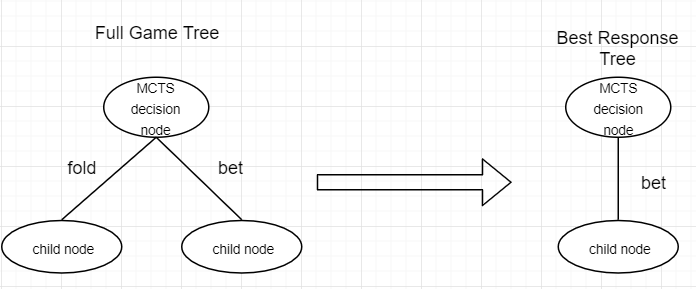
\includegraphics[scale=1]{images/best_response_tree_vs_full_tree.PNG}
    \caption{Generation of Best Response Tree}
\end{figure}

\subsection{Terminal Node Evaluation}\label{subsec:terminalNodeEvaluation}
The next step in this process is to evaluate the terminal nodes in the best response tree.
This process seems trivial on immediate inspection.
However, there is one important factor that must be considered.
That is that the BR player should not be allowed to choose different actions based on the
private information of the opponent.
This problem is avoided by calculating the average value of all histories that are equivalent in
the eyes of the BR player and applying this value to the terminal node that we are evaluating.
As an example, if the BR player has a king then the MCTS player may have a queen, a king, or an ace.
Each of these possibilities would result in a different value for the terminal.
Due to the fact that the BR player cannot see this information, they should not be able to vary
their behavior based on it.
As such we simply take all of these possibilities into account and assign the average value for
the terminal.
The code for this step is listed below.

\begin{lstlisting}[style=Python]
def evaluate_terminals(best_response_tree, terminals):
    for history in terminals:
        if history.endswith("f"):
            best_response_tree[history].value = gevaluator.calculate_reward(history)
        else:
            eq_nodes = util.get_information_equivalent_nodes(best_response_tree, history, -1)
            avg = evaluator.average_reward(eq_nodes)
            best_response_tree[history].value = avg
\end{lstlisting}

It is worth noting at this stage that although the self-play smooth UCT algorithm is utilising
stochastic strategies in training, the strategy evaluation step is evaluating a deterministic strategy.
This can be seen in the "apply\_mcts\_strategy" function listed above, where every
child aside from the highest valued child is being removed from the tree.
If the MCTS player's strategy was to be treated as a stochastic strategy then all child
nodes would be retained at this step.
Probabilities would be associated with each child depending on how often they had been visited during training.

When evaluating the exploitability of stochastic strategies one
modification to this step of the algorithm would be made.
A vector of reach probabilities\citep{johanson2011accelerating} would be calculated and these probabilities would
be applied across "information equivalent" terminal nodes for the BR player.
In other words, instead of simply averaging the return of these terminal nodes, they would be weighted.
For example, if $R$ is the reward function $p$ is a vector of reach probabilities and
$h^i$ is a vector of information equivalent nodes then the stochastic value would be:

\begin{align}
    v(h) = p_0*R(h_0) + p_1*R(h_1) + \dots + p_{n-1}*R(h_{n-1})
\end{align}

In contrast the deterministic evaluation is as follows:

\begin{align}
    v(h) = \dfrac{R(h_0) + R(h_1) + \dots + R(h_{n-1})}{n}
\end{align}

\subsection{Propagating Node Values}\label{subsec:propagateTerminals}
The final step of this process involves the propagation of values back up the tree, with the highest
child value being propagated when a decision node for the BR player is reached.
The average child value is propagated for chance nodes.
Since the MCTS player will only have a single child node for each history, that node's value is
propagated each time.
The code is listed below.

\begin{lstlisting}[style=Python]
def propagate_rewards_recursive(best_response_tree, history):
    parent = best_response_tree[history].parent

    if util.player(parent) == 0:
        value_to_propagate = util.get_average_child_value(best_response_tree, parent)
    elif util.player(parent) == 1:
        value_to_propagate = best_response_tree[next(iter(best_response_tree[parent].children))].value
    else:
        best_sibling = util.get_best_child(best_response_tree, parent, -1)
        value_to_propagate = best_response_tree[best_sibling].value

    best_response_tree[parent].value = value_to_propagate
    propagate_rewards_recursive(best_response_tree, parent)
\end{lstlisting}

\subsection{Exploitability}\label{subsec:exploitability}
When the process outlined is complete the value that is propagated back to the
root node is our exploitability value.

\section{Prototype Application}\label{sec:prototypeApp}
In order to give visual evidence of the work done and the agent developed, a user interface(UI) was created
that allowed human interaction with the trained bot.
In order to facilitate the development of this interface in a short period of time, the Qt framework was used.
Qt is an open source widget toolkit for creating graphical user interfaces and applications.
Specifically, Qt Designer was used in order to generate a UI template.
Qt Designer is a what-you-see-is-what-you-get (WYSIWYG) UI generation tool that accompanies Qt.
PyQt5 was then used to generate python code from this UI template and connect the functional component of the game.
In this section, the process involved in creating this prototype application will be outlined
and some key code snippets will be highlighted.

In order to elicit requirements for this application, I brainstormed as well as analysing a number
of online UIs that served a similar purpose to mine.
This process rendered the following functional requirements:

\begin{itemize}
    \item Display list of available actions.
    \item Allow user to take action.
    \item Display relevant cards to player.
    \item Annotate the sequence of events that occur in the game.
    \item Display the current pot size.
    \item Allow player to play multiple rounds.
    \item Keep track of cumulative winnings across multiple rounds.
\end{itemize}

\subsection{UI Screen}\label{subsec:UiScreen}
The first step towards achieving these functional requirements was to generate a UI screen.
This was achieved through Qt designer using drag and drop with the end result being as shown in figure 3.3.
Due to the fact that a number of images had to be displayed for the available cards in the
game a Qt resource file was also created to store and locate those images.

\begin{figure}[ht]
    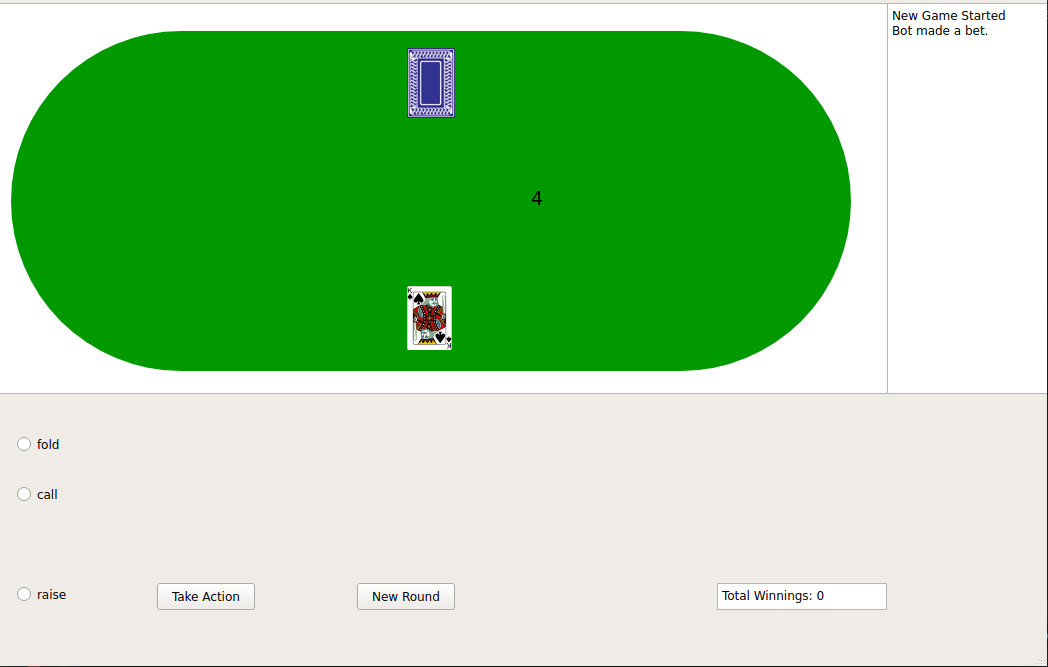
\includegraphics[scale=.4]{images/UI_screenshot.png}
    \caption{Game UI Screenshot}
\end{figure}

Qt designer generates a .ui file that stores the UI template as well as a .qrc resource file.
The following commands were used to convert these two files into python format in order for them
to be compatible with the rest of the program:
\begin{lstlisting}[language=bash]
$ pyuic4 -x ui.ui -o screen.py
$ pyrcc4 -o cards_resource.py cards/cards_resource.qrc
\end{lstlisting}

In order to create a visible screen the code listed below was used:
\begin{lstlisting}[style=Python]
def setup_screen(self):
    self.main_window = QMainWindow()
    self.ui_screen = screen.Ui_MainWindow()
    self.ui_screen.setupUi(self.main_window)
    self.main_window.show()
    sys.exit(self.application.exec_())
\end{lstlisting}

\subsection{Event Handling and UI Manipulation}\label{subsec:eventHandling}
When the UI screen had been implemented it was then time to attach the screen to the
functional aspect of the game.
This was done through the creation of a python class called Controller that extends the QWidget
class from the PyQt framework.

In order to handle events, callback methods were registered with the buttons that required their events to be handled.
The code listed below demonstrates this process:

\begin{lstlisting}[style=Python]
def setup_event_handlers(self):
    self.ui_screen.take_action_button.clicked.connect(self.take_action)
    self.ui_screen.new_game_button.clicked.connect(self.new_game)
\end{lstlisting}

Along with event handling the Controller class also had the responsibility of updating the
UI based on the information that it gained from the game model, which will be discussed in the next section.
This primarily involved calling the setText() method of a number of the screen's widgets.

\subsection{Game Model}\label{subsec:gameModel}
The third component of our game was the game model.
This was instantiated through a python class named Model that had the responsibility of feeding
the correct data to the Controller class at any point in the game.
Due to the fact that there was already significant functionality built around the concept of histories,
it was decided that the state of the game would be tracked through the use of histories.
From the history, the majority of the information about the game could be deciphered.
This included the available actions, the cards in play and the pot.
In order to fully satisfy our functional requirements, the Model class also kept track of annotation messages
that were generated based on game events, along with the cumulative winnings of the player over time.
This data was returned to the Controller class in the
form of a python dictionary.

The most significant method in this class was the update\_game\_state method.
This method handled the player taking actions, the agent responding to those actions and the state being
updated.
The code for this method is listed below.

\begin{lstlisting}[style=Python]
def update_game_state(self, action, player):
    self.history += action
    self.display_text += PLAYER_NAMES[player] + ACTION_MESSAGES[action]

    # Handle the game being over
    if util.terminal(self.history):
        winner = evaluator.get_winner(self.history)
        winnings = -evaluator.calculate_reward(self.history)
        self.total_winnings += winnings
        self.display_text += "Game over. " + PLAYER_NAMES[winner] + "won: " + str(abs(winnings))

    # If the next player is the bot, allow it to take its action
    elif util.player(self.history) == 1:
        self.update_game_state(self.agent.get_action(self.history), 1)

    # If the we need cards to be dealt, deal the cards.
    elif util.player(self.history) == 0:
        self.pub_card = random.choice(util.get_available_cards(self.history))
        self.update_game_state(self.pub_card, 0)
\end{lstlisting}

\subsection{Agent Representation}\label{subsec:agent}
In the case of this prototype game, the agent is merely an instantiation of a pre-defined strategy.
As such when we call agent.get\_action(history) in the previous code block we are either probabilistically
or deterministically selecting an action based on the aforementioned strategy.
Below we have listed the code for the Agent python class.
Lines 10 to 17 give the code that is executed in order to return an action if our strategy is stochastic.
Line 19 gives the code to return an action if the strategy is deterministic.

\begin{lstlisting}[style=Python]
class Agent:
    def __init__(self, strategy_file):
        self.strategy = load_strategy(strategy_file)

    def get_action(self, history):
        player_history = util.information_function(history, 1)

        # Is our strategy stochastic?
        if isinstance(self.strategy[player_history], dict):
            candidates = []
            probabilities = []

            for key, value in self.strategy[player_history].items():
                candidates.append(key)
                probabilities.append(value)

            return choice(candidates, p=probabilities)
        else:
            return self.strategy[player_history]
\end{lstlisting}

